\section*{Question 2}
(2.1) The ridge regression program written for question (1.3) is used to evaluate regression parameters for $\lambda$ = 1, 2, ..., 100. The prediction error computed on the test set is shown in Figure 4. The minimum value of error is approximately 209833 and is obtained when $\lambda$ = 2
\begin{figure}[h!]
    \centering
    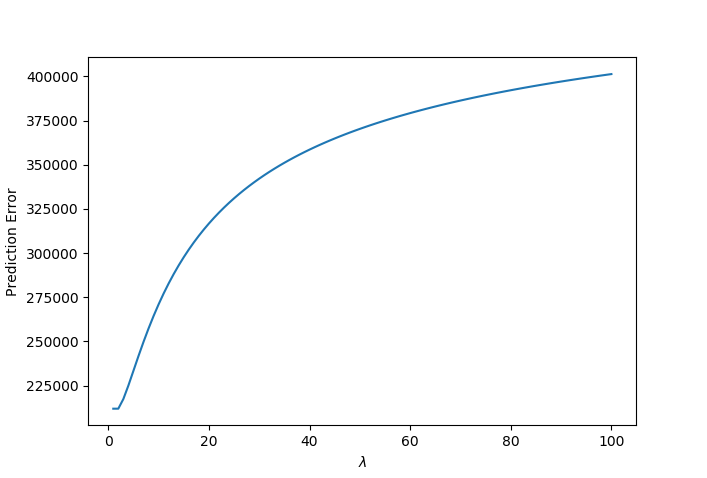
\includegraphics[height=4in]{Figure_4.png}
    \caption{Prediction error as a function of $\lambda$ for question (2.1)}
\end{figure}
\vspace{5mm}

(2.2) The program used to perform the kernel version of ridge regression is done for two cases:
\begin{enumerate}
    \item Gaussian kernel: $K(x, y)$ = exp$(-|x - y|^{2} / 2\sigma^{2})$
    \item Polynomial kernel of order $h$: $K(x, y) = \sum\limits_{k=1}^h (x^{T}y)^{k}$
\end{enumerate}
The prediction error for both cases is calculated using the following formula:
\begin{center}
    $\sum\limits_{l=1}^M|y_{l} - (\beta_{0} + \sum\limits_{k=1}^N\alpha_{k}K(x_{l}, x_{k}))|^{2}$
\end{center}
For the Gaussian kernel case and the polynomial kernel case with orders ranging from 1 to 4, the minimum values of the prediction error and the corresponding $\lambda$ values for are shown below in Table 1. For cases where the minimum error occurs over a range of values for $\lambda$, the range is listed below. Figures 5 - 9 show the prediction error as a function of $\lambda$ for all 5 cases.
\vspace{2cm}
\begin{table}[h!]
\centering
 \begin{tabular}{||c c c||} 
 \hline
 Case & $\lambda$ & Error \\ [0.5ex] 
 \hline\hline
Gaussian & 0.0025 - 0.1 & 495260 \\
Polynomial ($h$ = 1) & 1 - 100 & 490324 \\
Polynomial ($h$ = 2) & 100 & 509628 \\
Polynomial ($h$ = 3) & 100 & 913104 \\
Polynomial ($h$ = 4) & 100 & 2800327 \\ [1ex] 
 \hline
 \end{tabular}
 \caption{Estimates of prediction error and corresponding values of $\lambda$}
\label{table:1}
\end{table}
\begin{figure}[h!]
    \centering
    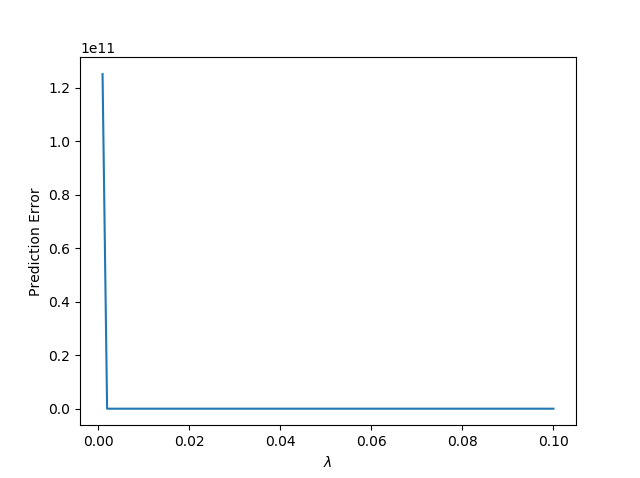
\includegraphics[height=3.5in]{Figure_5.png}
    \caption{Prediction error as a function of $\lambda$ for question (2.2) for the Gaussian kernel case}
\end{figure}
\begin{figure}[h!]
    \centering
    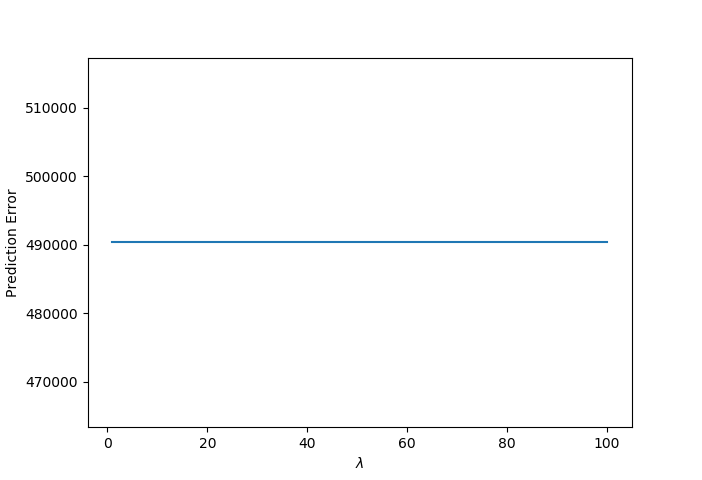
\includegraphics[height=3.5in]{Figure_6.png}
    \caption{Prediction error as a function of $\lambda$ for question (2.2) for the polynomial kernel case where $h$ = 1}
\end{figure}
\begin{figure}[h!]
    \centering
    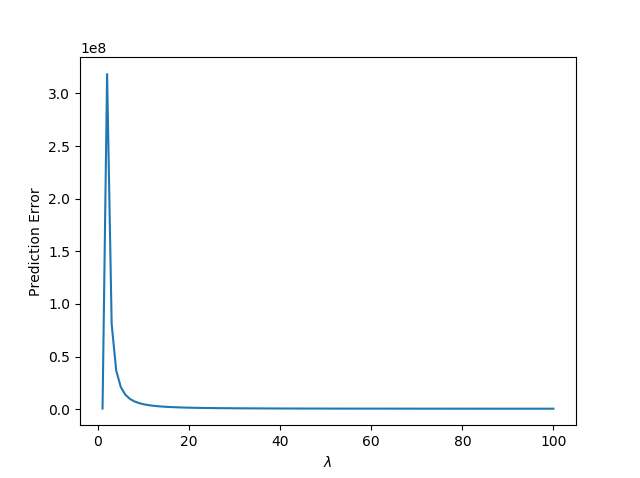
\includegraphics[height=3.5in]{Figure_7.png}
    \caption{Prediction error as a function of $\lambda$ for question (2.2) for the polynomial kernel case where $h$ = 2}
\end{figure}
\begin{figure}[h!]
    \centering
    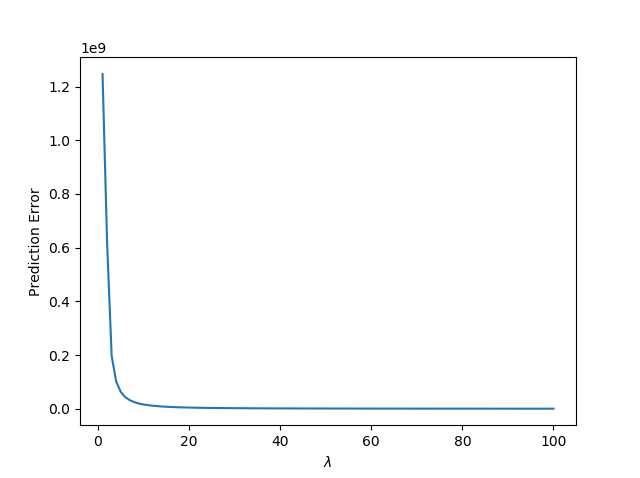
\includegraphics[height=3.5in]{Figure_8.png}
    \caption{Prediction error as a function of $\lambda$ for question (2.2) for the polynomial kernel case where $h$ = 3}
\end{figure}
\begin{figure}[h!]
    \centering
    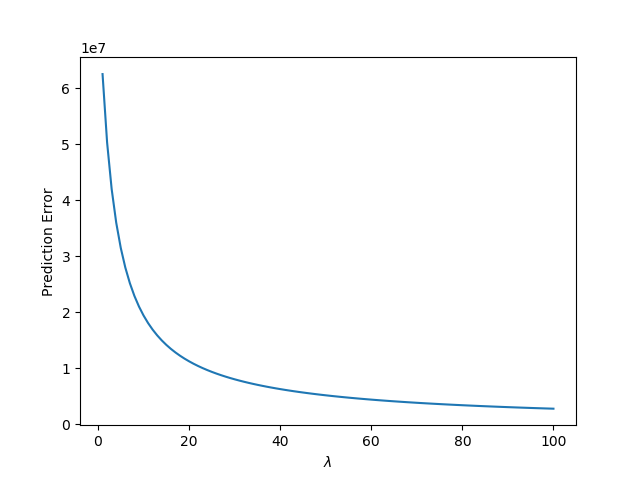
\includegraphics[height=3.5in]{Figure_9.png}
    \caption{Prediction error as a function of $\lambda$ for question (2.2) for the polynomial kernel case where $h$ = 4}
\end{figure}
\clearpage

(2.3) The results from the polynomial kernel case ($h$ = 2) should be identical to the linear one. The kernel for the second-degree polynomial is equivalent to the original expression as shown in the original error function to be minimized. In the actual results from the previous problem, the results do not match due to programming errors.